% $Id

%% Dokumentenklasse (Koma Script) -----------------------------------------
\documentclass[%
   %draft,     % Entwurfsstadium
   final,      % fertiges Dokument
	 % --- Paper Settings ---
   paper=a4,% [Todo: add alternatives]
   paper=portrait, % landscape
   pagesize=auto, % driver
   %twocolumn,
   % --- Base Font Size ---
   fontsize=10pt,%
	 % --- Koma Script Version ---
   version=last, %
 ]{scrartcl} % Classes: scrartcl, scrreprt, scrbook


% Encoding der Dateien (sonst funktionieren Umlaute nicht)
% Fuer Linux -> utf8
% Fuer Windows, alte Linux Distributionen -> latin1

% Empfohlen latin1, da einige Pakete mit utf8 Zeichen nicht
% funktionieren, z.B: listings, soul.

%\usepackage[latin1]{inputenc}
%\usepackage[ansinew]{inputenc}
\usepackage[utf8]{inputenc}
%\usepackage{ucs}
%\usepackage[utf8x]{inputenc}

\usepackage[T1]{fontenc}
\usepackage[english]{babel}

\addto\captionsenglish{
  \renewcommand{\contentsname}{Table of Contents}
}

\renewcommand{\rmdefault}{phv} % Arial
\renewcommand{\sfdefault}{phv} % Arial

\usepackage{appendix}
\usepackage{listings}
\usepackage{color}
\usepackage{geometry}
\usepackage{array}
\usepackage{graphicx}
\usepackage{caption}
%\usepackage{mathtools}
\usepackage{amsmath}

\usepackage{subcaption}
%prefer subcaption instead of subfigure
%\usepackage{subfigure}

\usepackage{float}

%\usepackage{algorithmic}
\usepackage{amstext}
\usepackage{tikz}
\usetikzlibrary{arrows,decorations.pathmorphing,fit,positioning}

\newcommand{\dir}{\text{Dirichlet}}
\newcommand{\mult}{\text{Multinomial}}

%\usepackage{hyperref}

\sffamily

%% Titel -----------------------------------------
\title{Topic Detection and Tracking System}
\subtitle{Research Project Master Artificial Intelligence Group 5}
\author{Daniel Brüggemann\\Yannik Hermey\\Carsten Orth\\Darius Schneider\\Stefan Selzer}

%% Dokument -----------------------------------------
\begin{document}

\maketitle
\thispagestyle{empty}
\newpage

\tableofcontents
\newpage



\section{Introduction}\label{sec:Introduction}

Growth of internet came along with an increasingly complex amount
of text data from emails, news sources, forums, etc. As a consequence,
it is impossible for a single person to keep track of all relevant text
data in most cases and moreover to detect changes in trends or
topics.
\\
\\
Every company (and every person) would be interested to harness
this amount of free and cheap data in order to develop intelligent
algorithms, which are able to react to emerging topics as fast as
possible and at the same time track existing topics over long time
spans. There are many techniques about topic extraction (like Nonnegative
Matrix Factorization (NMF) or Latent Dirichlet Allocation
(LDA) \cite{Blei:2003:LDA:944919.944937} ) but there are not many extensions to dynamic data
handling.
The goal of this project is to explore LDA (or other techniques) as a
technique to detect topics as they appear and track them through
time. Corpus can be the (fully annotated and immediately available)
RCV1 Reuters corpus (810.000 documents) and/or the actual
Reuters archive.

\section{State Of The Art}\label{sec:SOTA}

This section gives an overview of the technical approaches currently used in the field of topic detection and tracking. First the approaches to preprocess the document dataset are described. Then the general tasks, that have to be performed to detect and track topics over time, are presented. Finally the two major approaches, namely Latent Dirichlet Allocation and non-negative matrix factorization, are presented.

\input{./tex/Preprocessing.tex}

\subsection{Topic Detection and Tracking Tasks}\label{sec:TDT}
The topic detection and tracking tasks according to \cite{Fiscus:2002:TDT:772260.772263} are as follows:
\begin{itemize}
	\item Topic Tracking: Track an identified topic over a period of time.
	\item Link Detection: Detect links between topics at different time points.
	\item Topic Detection: Identify different topics.
	\item First Story Detection: Identify the first occurence of a certain topic in the timeline.
	\item Story Segmentation: Identify splitting of topics into new ones and the corresponding points in time.
\end{itemize}

Some of these tasks are reflected in the approaches presented in the following sections and some have to be considered in addition to the given implementations.

\subsection{Latent Dirichlet Allocation}\label{sec:LDA}

Latent Dirichlet Allocation (LDA) \cite{Blei:2003:LDA:944919.944937}
 is a generative probabilistic mixture model for topic detection. In such a model, text is represented as a set of words (bag-of-words). Grammar and word order are disregarded while multiplicity, i.e. the frequency of occurences of single words in the text, is being kept and can be used as feature for topic detection. Words define a vocabulary and topics are represented by a probabilistic distribution of words from this vocabulary. Each word may be part of several topic representations. LDA asumes that each document from a collection of documents is generated from a probabilistic distribution of topics. The model tries to infer these probabilistic distributions by maximizing the probabilities of the words given the topic distribution. This means, that the words in a certain document are generated by first choosing a topic from the topic distribution and then choosing a word from that topic such that the probability of that word given that topic is maximized. As the actual computation of the probabilities is intractable, the posterior probability of a word given a topic is computed iteratively using sampling methods. Blei et al. \cite{Blei:2003:LDA:944919.944937} use Bayes' Theorem in combination with a Dirichlet distribution as prior distribution to approximate the true posterior distribution. The probability space defined by the probabilites of the words and topics is multidimensional which is represented by a multinomial distribution. For the a priori estimation the conjugate distribution is needed, which corresponds to a Dirichlet distribution in this case. Information gain is used as measure for the difference between two iterated probability distributions and thereby acts as convergence criterion.
%\\
%The parameter estimation for a correct setup of the initial distributions needs to be investigated further here.

\begin{figure}[htp]
  \centering
  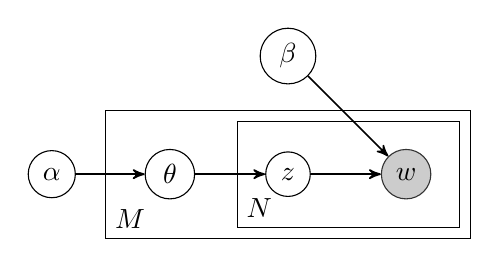
\begin{tikzpicture}
    [
      observed/.style={minimum size=15pt,circle,draw=black!80,fill=black!20},
      unobserved/.style={minimum size=15pt,circle,draw},
      post/.style={->,>=stealth',semithick},
    ]

    \node (w) [observed] at (0,0) {$w$};
    \node (z) [unobserved] at (-1.5,0) {$z$};
    \node (z-prior) [unobserved] at (-3,0) {$\theta$};
    \node (z-hyper) [unobserved] at (-4.5,0) {$\alpha$};
    \node (w-hyper) [unobserved] at (-1.5,1.5) {$\beta$};

    \path
    (z) edge [post] (w)
    
    (z-hyper) edge [post] (z-prior)
    (z-prior) edge [post] (z)

    (w-hyper) edge [post] (w)
    ;

    \node [draw,fit=(w) (z-prior), inner sep=14pt] (plate-context) {};
    \node [above right] at (plate-context.south west) {$M$};
    \node [draw,fit=(w) (z), inner sep=10pt] (plate-token) {};
    \node [above right] at (plate-token.south west) {$N$};

  \end{tikzpicture}
  \caption{Plate diagram representing LDA as a Bayesian network. The outer box represents M documents, the inner box represents the N times repeated choice of topics and words within a document. $\theta$ represents the topic distribution per document. $\alpha$ and $\beta$ represent the concentration parameters for the per-document and per-topic Dirichlet distributions. The variable $w$ is observable while the other variables are latent. Edges denote dependencies among variables. \cite{Blei:2003:LDA:944919.944937} }
  \label{fig:lda}
\end{figure}

There are extensions of the LDA model towards topic tracking over time, as \cite{Wang:2006:TOT:1150402.1150450} and \cite{conf:ijcai:WeiSW07}. But according to \cite{conf:uai:WangBH08}, these methods deal with constant topics and the timestamps are used for better discovery. Opposed to that, in \cite{conf:uai:WangBH08} a model for detection of evolving topics in a continuous time is presented. This is an extension of the model working on discrete time space presented in \cite{Blei:2006:DTM:1143844.1143859}. Here LDA is used on topics aggregated in time epochs and a state space model handles transitions of the topics from one epoch to another, together with a gaussian probabilistic model to obtain the posterior probabilities on the evolving topics along the timeline. The continuous model can be seen as the limit of this discrete model with finest possible granulation regarding the time steps. To deal with the exceptionally increasing computational resources required in this case, the probabilistic model is exchanged by a Brownian motion, which represents the limiting process of a discrete-time Gaussian random walk \cite{Blei:2006:DTM:1143844.1143859}. In addition advantage is taken of the sparsity of the topic distribution in time.



%Document consists of N different words from a vocabulary of size V, where each word corresponds to one of K possible topics.
%The posterior probability is computed using Bayes' Theorem:
%
    %$P(A\mid B) = \frac{P(B \mid A)\, P(A)}{P(B)}\cdot \, $
		%
%Mixture model with multinomial distribution with only one trial which is formally equivalent to the categorical distribution.\\
%
%Topic model as a mixture of K different V-dimensional distributions.
%Prior distribution using conjugate of multinomial distribution, Dirichlet.
%\\
%Observable and latent (hidden) variables.
%Bayesian network (directed acyclic graph) to describe conditional dependencies of random variables.
%\\
%\\
%The generative process is as follows. Documents are represented as random mixtures over latent topics, where each topic is characterized by a distribution over words. LDA assumes the following generative process for a corpus $D$ consisting of $M$ documents each of length $N_i$:
%\begin{enumerate}
	%\item Choose $\theta_i \, \sim \, \mathrm{Dir}(\alpha)$ , where $i \in \{ 1,\dots,M \}$ and $\mathrm{Dir}(\alpha)$ is the Dirichlet distribution for parameter $\alpha$
	%\item Choose $\varphi_k \, \sim \, \mathrm{Dir}(\beta)$ , where $k \in \{ 1,\dots,K \}$
	%\item For each of the word positions $i, j$ , where $j \in \{ 1,\dots,N_i \}$ , and $i \in \{ 1,\dots,M \}$
	%\begin{enumerate}
		%\item Choose a topic $z_{i,j} \,\sim\, \mathrm{Multinomial}(\theta_i)$.
		%\item Choose a word $w_{i,j} \,\sim\, \mathrm{Multinomial}( \varphi_{z_{i,j}})$.
	%\end{enumerate}
%\end{enumerate}
%
%The lengths $N_i$ are treated as independent of all the other data generating variables ($w$ and $z$). The subscript is often dropped, as in the plate diagrams shown here.

%\begin{algorithmic}[1]
%  \FOR{document $d_d$ in corpus $D$}
%  \STATE Choose $\theta_d \sim \dir(\alpha) $
%  \FOR{position $w$ in $d_d$}
%    \STATE Choose a topic $z_w \sim \mult(\theta_d)$
%    \STATE Choose a word $w_w$ from $p(w_w | z_w,\beta)$, a multinomial distribution over words conditioned on the topic and the prior $\beta$.
%  \ENDFOR
%  \ENDFOR
%\end{algorithmic}


%Dirichlet with a concentration parameter alpha significantly below 1 to concentrate the probability mass in few components and encourage sparse distributions, i.e. only a small number of words have significantly non-zero probabilities.


\subsection{Non-Negative Matrix Factorization}\label{sec:NMF}

Non-negative matrix factorization is an algorithm that can be used in the field of text mining to factorize and thereby decrease the dimension of a large matrix \cite{Lee}. For topic detection, the original matrix can be composed of terms represented by the rows and documents represented by the columns. The cell values typically represent the number of occurrences of a word in a document. As this value cannot be negative, the algorithm's requirement of a matrix with only non-negative values is fulfilled. This matrix is then factorized into two positive matrices which have significantly lower dimensions, one representing a term-feature relation, the other one representing a feature-document relation. \\
The new matrices' features are hidden and might represent correlations not visible before. When multiplied with each other, these matrices form an approximation of the original matrix and fill in zero-values, acting as predictors for the cell values.\\

Advantages of this algorithm are storage savings due to the sparsity of factorization and the good scalability for increasing matrix dimensions. Disadvantages are that the factorization is not unique and convergence is not always guaranteed.\\
Although the original data size can be too large for matrix factorization, there already exist variants of the algorithm using an dynamic approach, processing data in chunks \cite{NMFOnline}. A dynamic and online processing of web articles using NMF is thus feasible.


\section{Existing Software Frameworks}\label{sec:software}

This section gives an overview of existing implementations for the modules of the topic detection and tracking system.

\subsection{LDA Implementation by Blei}

Among the various implementations provided by David Blei and his group at Columbia University there is also a ready-to-use application\footnote{https://github.com/Blei-Lab/dtm} corresponding to the dynamic model described in \cite{Blei:2006:DTM:1143844.1143859}. The programming language is C as for most of the original work. Unfortunately there is no implementation for the continuous extension. As a drawback the documentation is very sparse.

\subsection{NMF Implementation LIBNMF}

A library implementing non-negative matrix factorization is available in the programming language C, called LIBNMF, which provides a number of variations of the algorithm. \cite{NMFSoftware} can serve as documentation.

\subsection{Java Library for Machine Learning}

There is also a Java library available covering multiple algorithms and techniques in the field of machine learning, including both LDA and NMF \cite{MLSoftware}. Documentation and examples how to use the algorithms can be found directly on sourceforge.net/projects/jlml/files/JML/. It has to be determined whether the algorithms are configurable to the needs of the project's problem domain (dynamic tracking of topics).

\subsection{JGibbLDA / GibbLDA++}
GibbLDA is a framework implemented in Java or C, which is based on the LDA algorithm and Gibbs sampling. Functionality for information retrieval, document classification, collaborative filtering and content-based image Clustering are provided by this library and might be very useful in the matter of topic detection. It is able to handle large databases and was successfully applied to fractions of wikipedia. 
\section{Corpus}\label{sec:Corpus}

Some words on the datasets
\section{Work plan}\label{sec:plan}

This sections describes the work plan for this project and the time frame for the work packages over the periods of this semester.

\begin{enumerate}
	\item Get an understanding of the technical background. \label{plan:step:research}
	\item Identify possible solutions for
	\begin{itemize}
	    \item Text preprocessing/normalization,
		\item Topic detection and tracking,
		\item Visualization.
	\end{itemize}
	\item Find applicable software frameworks. \label{plan:step:find}
	\item Clarify interfaces of software frameworks. \label{plan:step:clarify}
	\item Implement requirements to make use of the frameworks.
	\item Apply the frameworks using the given data set.
	\item Verify and enhance the results, go back to step \ref{plan:step:clarify} if necessary. \label{plan:step:enhance}
	\item Consolidate the results.
\end{enumerate}

The steps \ref{plan:step:research} to \ref{plan:step:find} are considered to be finished by the end of the first period. The steps \ref{plan:step:clarify} to \ref{plan:step:enhance} are planned for the second period. In the final period the consolidation will finish the actual project work and form the foundation for the final report.

% Bibliography:
%\clearpage
\addcontentsline{toc}{section}{Bibliography}

\bibliographystyle{apalike}
\bibliography{./tex/report}

\end{document}
